\section{Modes of Parallel Execution}

%%, potentially using commodity hardware

Parallelism in test execution can be obtained at different levels.
Figure~\ref{fig:levels} illustrates some of these levels.  This paper
focuses at lower-level parallelism, obtained with parallel computation
at cpus and threads in a given machine.  This kind of parallelism is
enabled through build systems and testing frameworks.  Given the
proliferation of multicore machines it is not surprising that testing
frameworks provide today support for parallel test execution with the
goal of running tests more efficiently~\cite{junit-org,testng,nunit}.
Build systems wrap the features of these frameworks to facilitate the
use of such technology\cite{maven-surefire-plugin}.  In the following
we elaborate relevant features of these components focusing on Java,
Maven, and JUnit but the discussion can be generalized to other
languages, build systems, and testing frameworks.

Note that lower-level parallelism is a complement to higher-level
parallelism that could be enabled through server farms.  For the
scenario of large IT organizations, lower-level parallelization
schemes could leverage the computing power of server nodes in addition
to the aggregate processing power of the farm.  Lower-level
parallelism fits particularly well smaller organizations (/projects)
with relatively high testing costs but lower budgets.
\Comment{Unfortunately, these solutions can't be used out-of-the-box:
  unrestricted parallel execution of tests can produce
  non-deterministic results as developers typically do not provision
  protection to concurrent accesses originated from arbitrary program
  points (\ie{}, tests).  We refer to this problem as Parallel
  Execution Flakiness (\pef{}).}

%% These solutions enable the
%% use of commodity hardware to maximize CPU usage\footnote{In the case
%%   of the Java language, for example, it is possible to explore
%%   parallelism across and within JVMs.}.  

\Comment{
To illustrate the importance of parallel test execution and
the problem of \pef{} let's consider the case of the ``core'' module
from the Apache Camel project~\cite{apache-camel-web}.  This module
contains 5,679 test cases, declared in 2,356 test classes.  We ran
those tests in a machine with 16GB of memory and 8 virtual CPUs (4
cores with 2 native threads each).  Sequential test execution takes
24m50s to run this test set.  Execution of the same test set takes
2m28s when we configured parallel execution to fork a JVM per CPU and
execute test classes, uniquely allocated to that JVM, sequentially but
running test methods from each class in separate threads.  Note that
this is an order of magnitude speedup (10.07x)\Fix{Need to understand
why this is 10x as opposed to something closer to 7x - I didn't get
your concern here}.  Unfortunately, due to \pef{}, $\sim$2\% (114 of
5,679) of the tests fail when executed in parallel.  It is important
to notice that the ratio of failures varies with the project as it
depends on factors such as length of test cases and amount of shared
state across tests.

\pef{} is an important obstacle to enable parallel test execution.
Conceptually, higher parallelization can result in higher chances of
concurrency-related problems.  It is important to execute tests
efficiently without sacrificing reliability
\Fix{gap between pars?? What gap?}

}



\subsection{Build Systems}
Build systems, such as Maven\footnote{\url{maven.apache.org}},
typically provide the option to \emph{fork} JVM instances
proportionally to available cores in the machine.  If the option
``fork JVM'' is enabled, Maven will allocate a user-provided number of
JVM instances to each core in the machine and will allocate each test
class to exactly one JVM.  Note that there is no guarantee to
uniformly distribute load to each JVM given that the build system uses
classes as the unit to specify test tasks.\Fix{we need to know how
  Maven allocates test classes to JVMs}

\subsection{Testing Framework}

The list below shortly describes the choices to control parallelism
within each JVM.

\begin{figure}[t!]
  \centering
  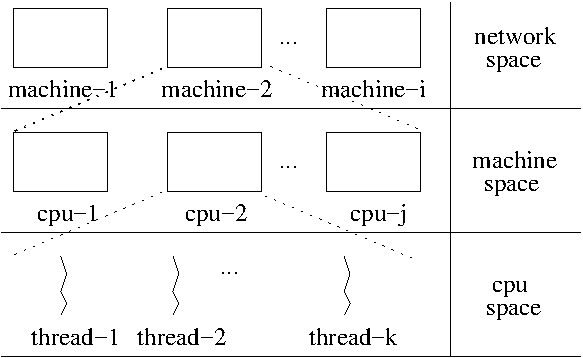
\includegraphics[width=0.4\textwidth]{figs/parallel-levels.pdf}
  \caption{\label{fig:levels}Levels of parallelism.}
\end{figure}

\newcommand{\Seq}{L0}
\newcommand{\ParClassSeqMeth}{L1}
\newcommand{\SeqClassParMeth}{L2}
\newcommand{\ParClassParMeth}{L3}

\begin{itemize}
\item \textbf{Sequential (\Seq).}~This configuration results in
  sequential execution of test classes and their methods, according to
  the order defined in the testing framework\Fix{cite}.  For JUnit
  this is the default configuration.
\item \textbf{Sequential classes; parallel methods
  (\ParClassSeqMeth{}).} This configuration results in the sequential
  execution of the test classes assigned to the JVM.  However, within
  each class, test methods run in parallel.\Fix{are there options to
    limit number of threads or a thread per test method?  Do they use
    thread pools?  etc....}
\item \textbf{Parallel classes; sequential methods
  (\SeqClassParMeth{}).}  This configuration results in the parallel
  execution of test classes but test methods of any given class are
  executed sequentially.\Fix{one thread per class?  if not, what
    classes are scheduled to execute first?}
\item \textbf{Parallel methods (\ParClassParMeth).} This configuration
  results in parallel execution of any given test method of any class.
\end{itemize}

\Fix{We need a par. providing rationale in to explain (points in favor/against) these choices.}
